\documentclass[12pt]{beamer}
\usetheme{LMT}
\usepackage[utf8]{inputenc}
\usepackage{amsmath}
\usepackage[makeroom]{cancel}
\usepackage{xcolor}

\setbeamertemplate{footline}[frame number]{}

\newcommand\Ccancel[2][black]{\renewcommand\CancelColor{\color{#1}}\bcancel{#2}}

\pdfinfo
{
  /Title       (Presentation Reunion)
  /Author      (Pierre NARGIL)
}

\newcommand\FontReduce{\fontsize{8}{10}\selectfont}
\newcommand\FontReduceT{\fontsize{9}{11}\selectfont}


\title{Avancement du travail}
\subtitle{Présentation hebdomadaire}
\author{Pierre Nargil}

\graphicspath{{figures/}}
% ---------------------------------------------------------------------
\begin{document}


\frame{\titlepage}

\frame{\tableofcontents}


\section{Rappels de la dernière réunion}

	\begin{frame}
	
		\frametitle{Rappels de la dernière réunion}
		%\framesubtitle{Un sous titre}
		
		\begin{itemize}
%			\item Les questions abordées :
%			\begin{itemize}
%				\only<1>{\FontReduce}
%				\item Expliquer la différence sur le cas analytique
%						\\ 	\only<2>{\textcolor{blue}{Évolution du programme de François depuis la présentation.}}
%				\item \textcolor<-1>{red}{Pour réutiliser les modes trouvés par SVD, comment trouver les fonctions en temps associées ?}
%						\\ 	\only<3>{\textcolor{blue}{...}}
%				\item \textcolor<-1>{red}{Le 1er mode de la 1ère itération est-il  la répose statique dde l'effort moyen ?}
%			\end{itemize}
			
			\only<-1>{
				\item Les objectifs de travail à court terme :
				\begin{itemize}
					\FontReduce
					\item \textcolor<-1>{red}{Differente fréquences F(t) (comparer aux f propre de la poutre) $\Rightarrow$ quand ça diverge
							(Somme de sinus à la place de SinusVerse ?)}
					\item \textcolor<-1>{red}{SVD(Solution PGD) - Mettre la SVD dans la boucle CalcMode}					
				\end{itemize}
			}
		\end{itemize}

	\end{frame}

%\section{Point de travail - avancement}

%\section{Questions soulevées}
\section{Constats et Remarques}
	\begin{frame}
	\FontReduceT
		\frametitle{Constats et Remarques}
		\begin{itemize}
			\only<1>{
			\item Les résultats pour cas Sinus/SinuVerse - Différents schémas - Différentes périodes de chargement
				\begin{itemize}
					\FontReduce
					\item Sans amortissement, $T_{propre}$:  / $3.86e^{-4}$ / $1.30e^{-4}$ / $ 7.76e^{-5}$ 
																						/ $ 5.48e^{-5}$ / $ 4.24e^{-5}$ / $3.48e^{-5}$ s
					\item $T_{charge}$:  $40$ / $60$ / $80$ / $120$ / $160$ / $200$ / $250$ $e^{-6}$s
					\item Beaucoup de divergence à partir d'un certain nombre de modes - et stagnation sinon
					\item Tout s'améliore avec un $dt$: $4e^{-6}\Rightarrow 1e^{-6}$ ??
				\end{itemize}
				}
			
			\only<2>{
			\item Les résultats sur masse-ressort cas SinuVerse - Différents amortissements et schémas
				\begin{itemize}
					\FontReduce
					\item $\xi = 0.7$
						\begin{itemize}
							\FontReduce
							\item Schéma 3 $\Rightarrow$ Convergence
							\item Schéma 4 et 5 $\Rightarrow$ Stagnation à $10^{-2.7}$
						\end{itemize}
					\item $\xi = 0.9$ (même en changeant $\alpha$)
						\begin{itemize}
							\FontReduce
							\item Schéma 3 $\Rightarrow$ ?
							\item Schéma 4 $\Rightarrow$ Convergence
							\item Schéma 5 $\Rightarrow$ Stagnation à $10^{-2.7}$
						\end{itemize}
					\item $\xi = 0.9$ (même en changeant $\alpha$)
						\begin{itemize}
							\FontReduce
							\item Schéma 3 $\Rightarrow$ ?
							\item Schéma 4 $\Rightarrow$ Convergence - Plus lente
							\item Schéma 5 $\Rightarrow$ Convergence très lente $10^{-0.8}$ à 20 modes
						\end{itemize}
				\end{itemize}
			\item Augmentation de l'amortissement sur problème poutre $\Rightarrow$ pas de résolution PGD.
				}
				
			\only<3-5>{
				\item Implémentation de la SVD dans le calcul des Modes
				\begin{itemize}
					\FontReduce
					\item Codes trouvés incorrect - trop grand $\Rightarrow$ calcul de $g(t)$
				\end{itemize}
				}
			\only<3>{
			\begin{figure}
				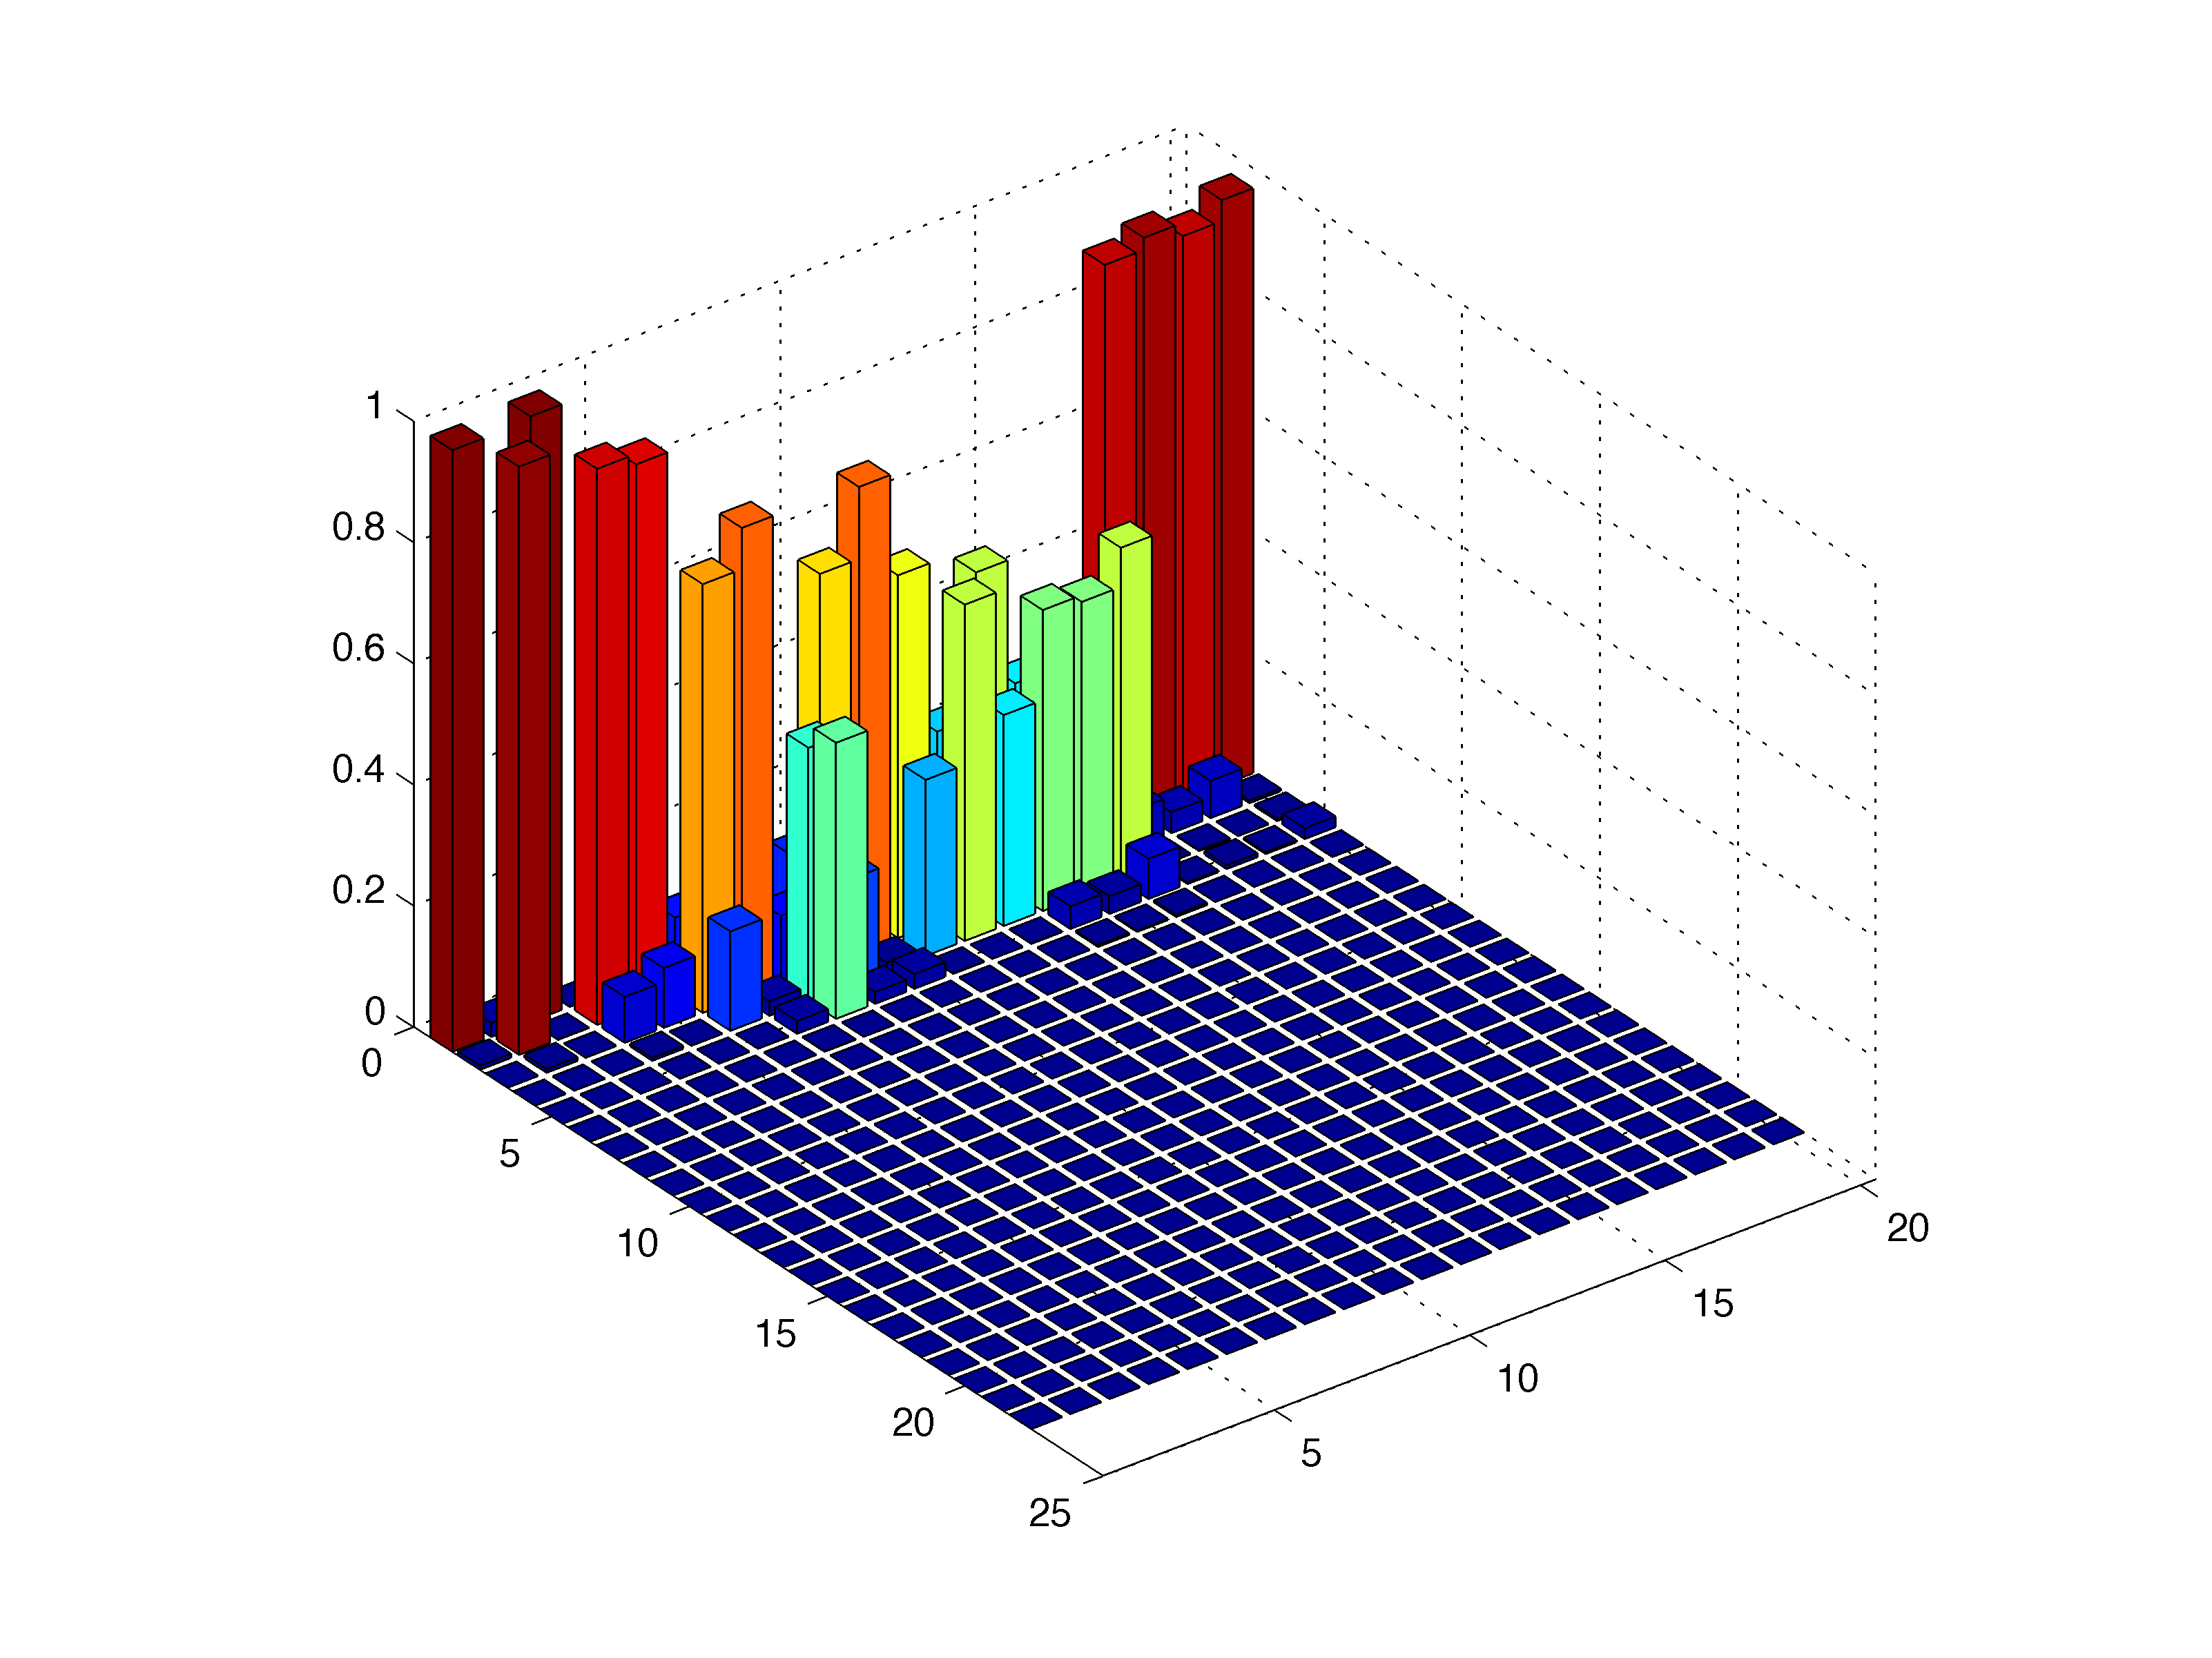
\includegraphics[width=0.5\linewidth ,keepaspectratio]{MAC_POD-PGD-Avant.png}				
				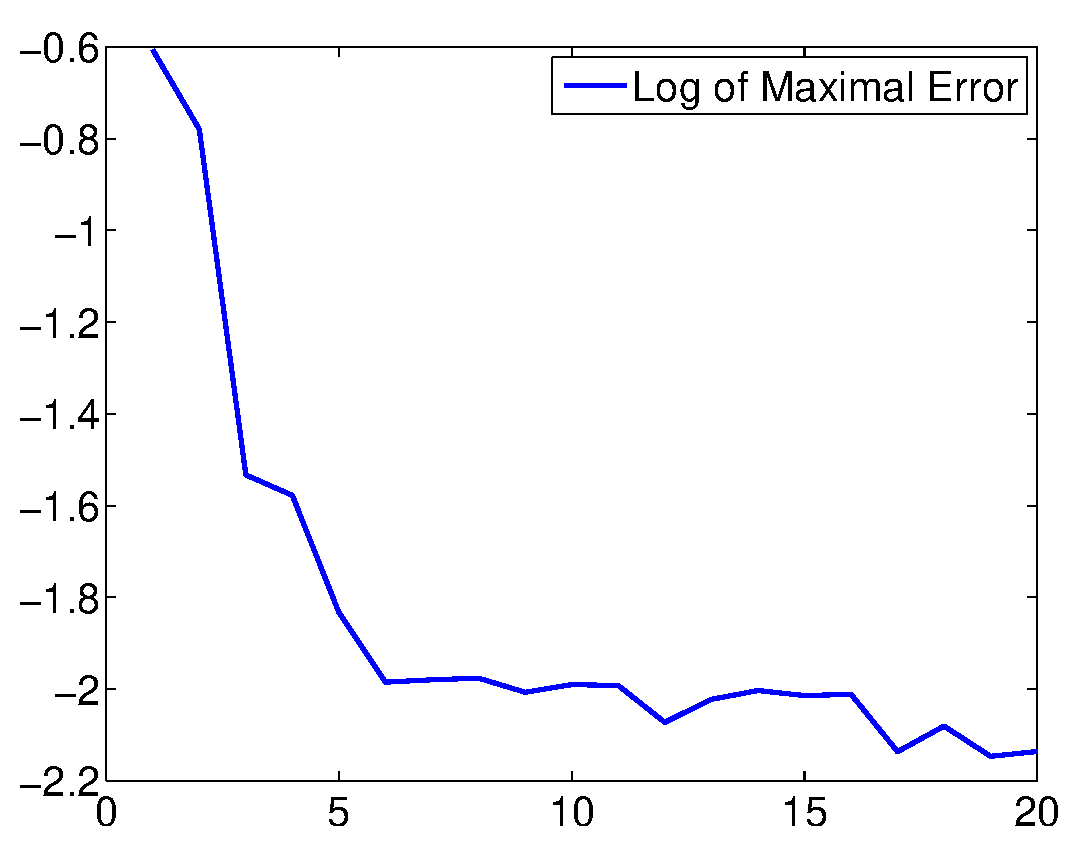
\includegraphics[width=0.5\linewidth ,keepaspectratio]{matPGDErreur-Avant.eps}	
			\end{figure}
			}
			\only<4>{
			\begin{figure}
				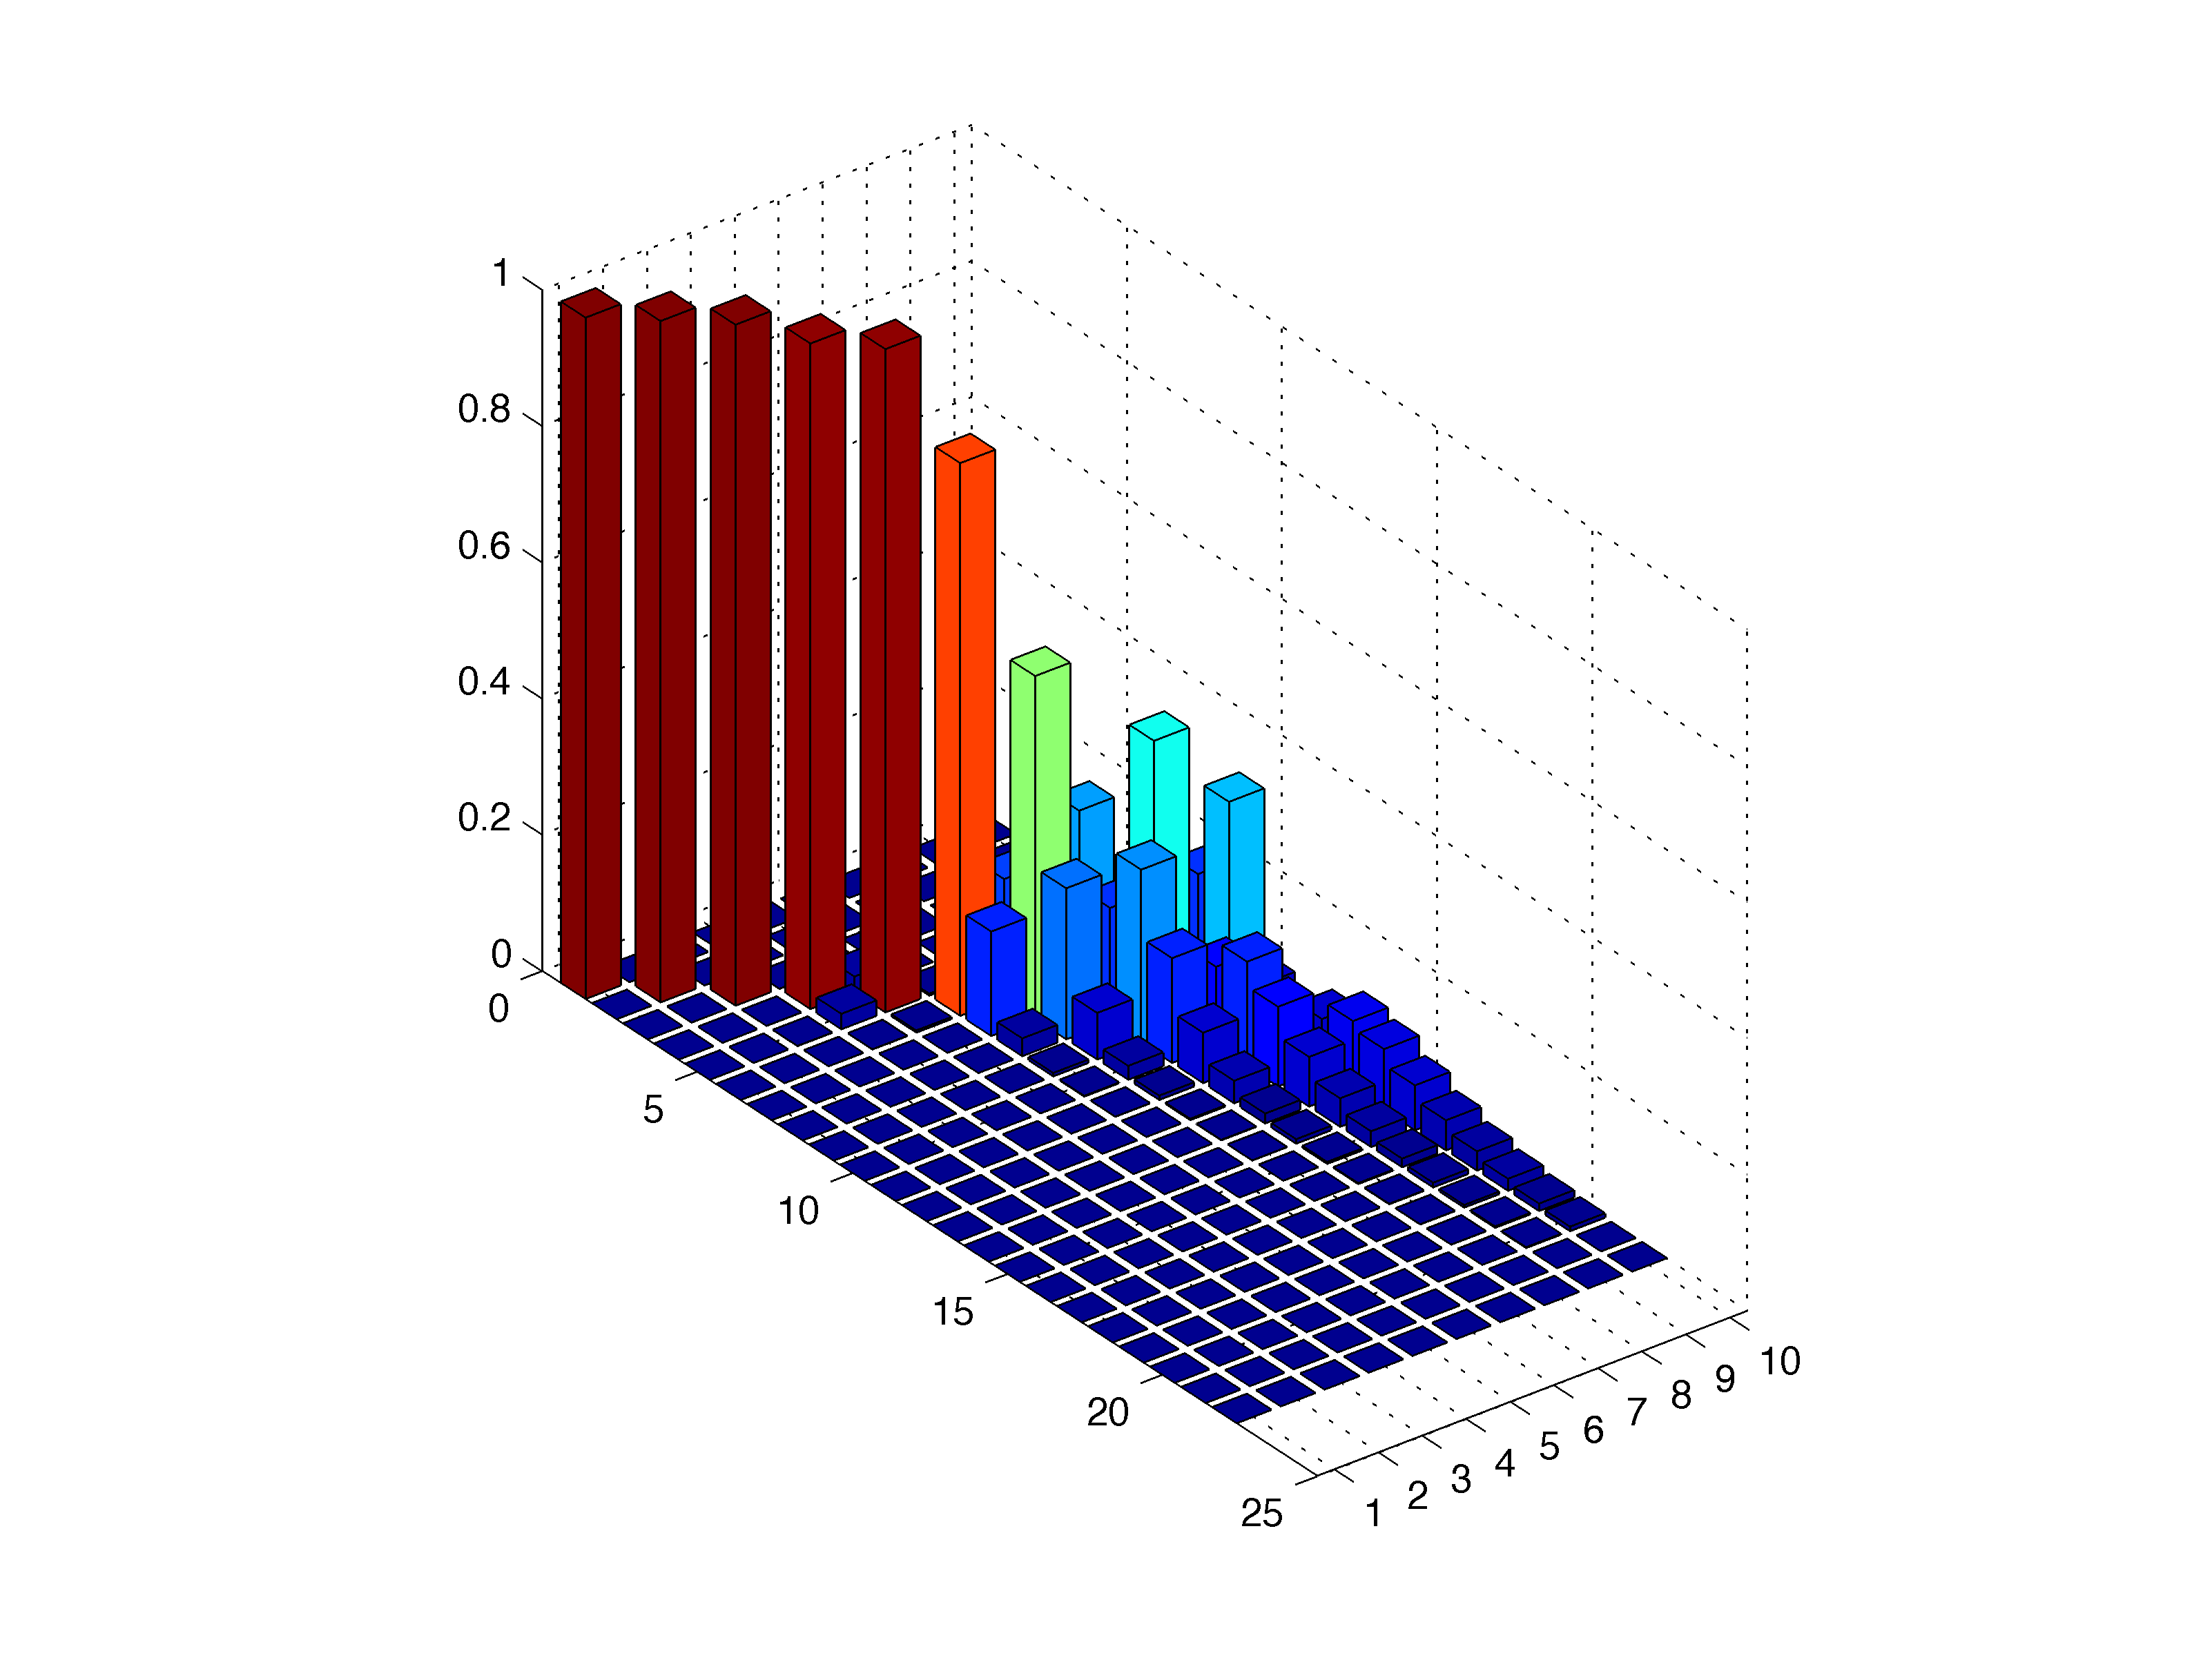
\includegraphics[width=0.5\linewidth ,keepaspectratio]{MAC_POD-PGD-apres.png}				
				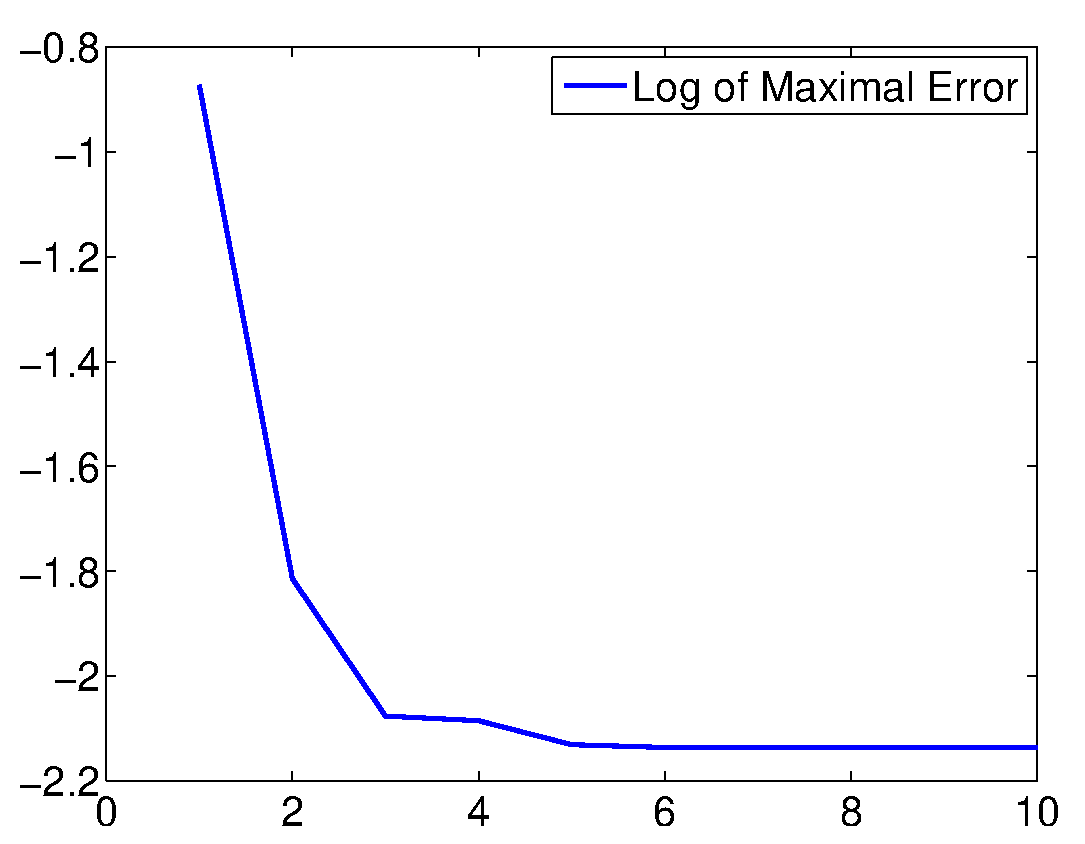
\includegraphics[width=0.5\linewidth ,keepaspectratio]{matPGDErreur-apres.eps}	
			\end{figure}
			}
			\only<5>{
			\begin{figure}
				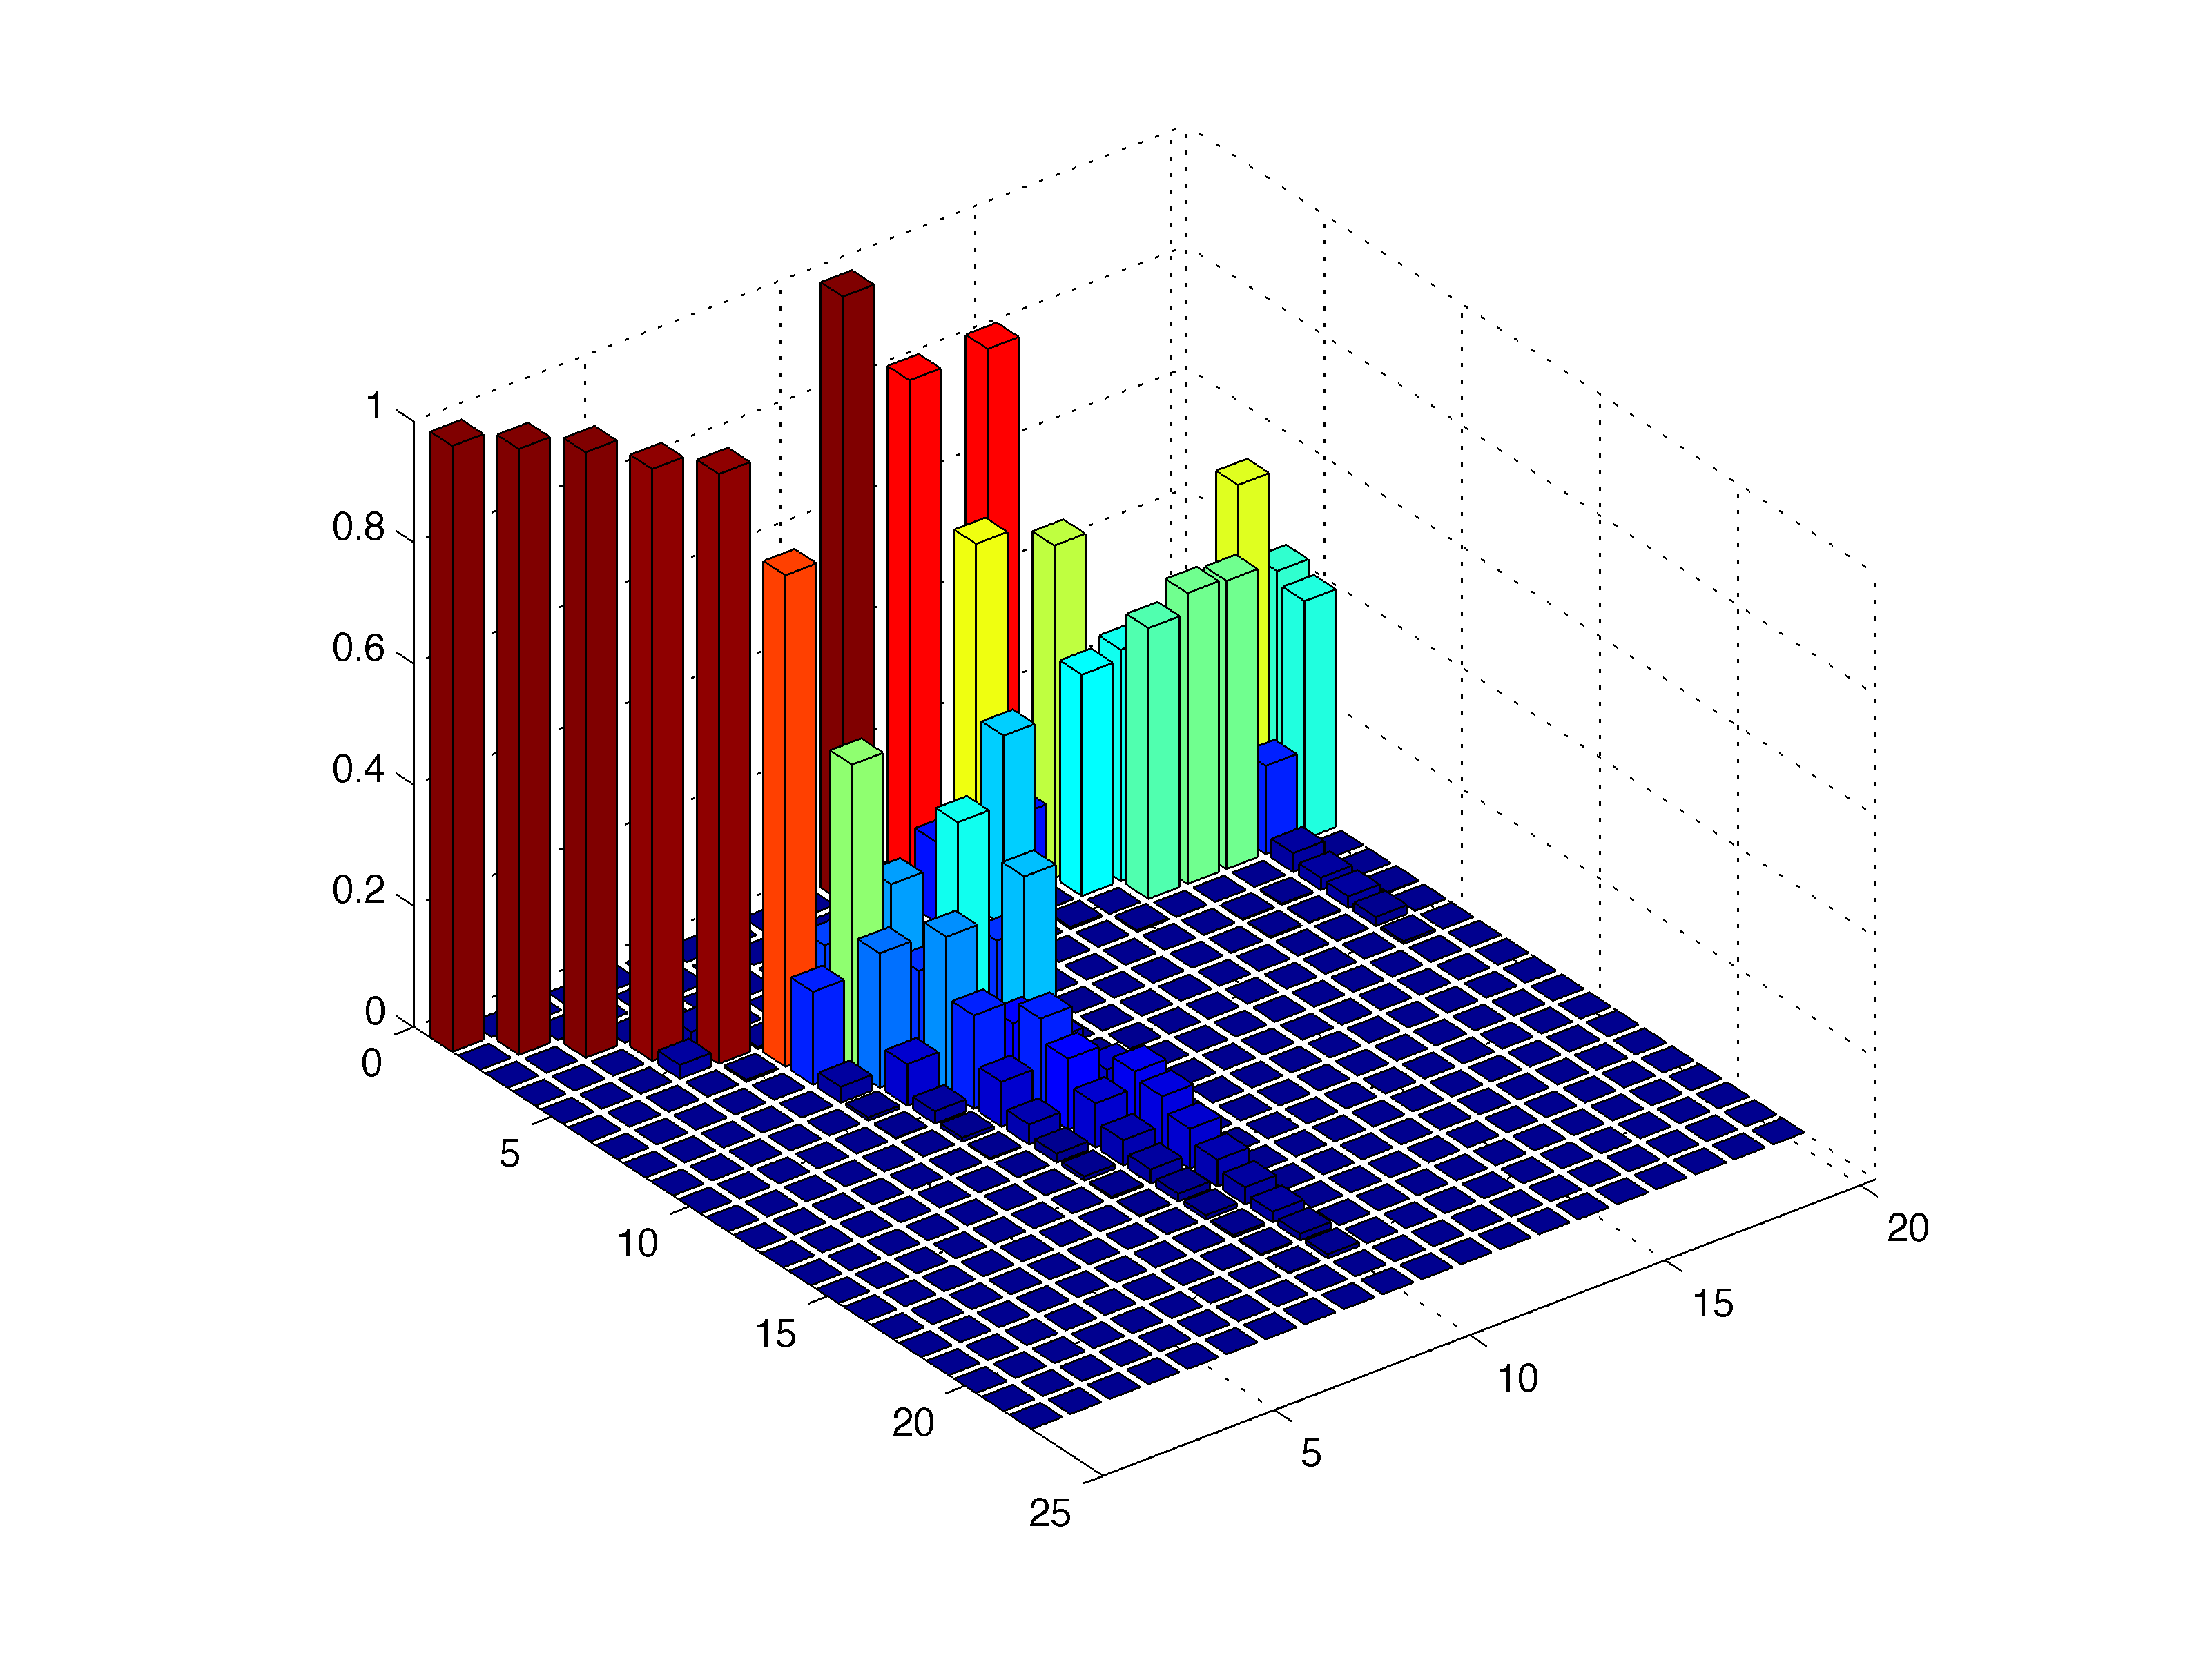
\includegraphics[width=0.5\linewidth ,keepaspectratio]{MAC_POD-PGD-continu.png}				
				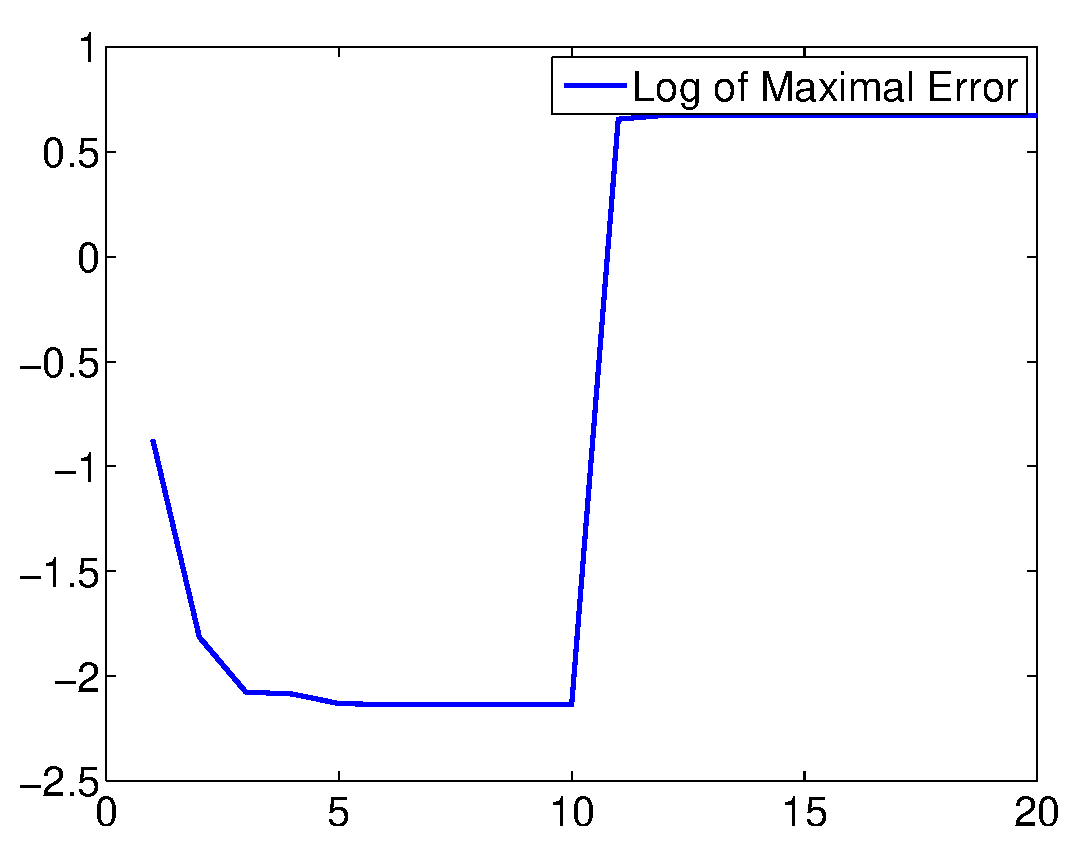
\includegraphics[width=0.5\linewidth ,keepaspectratio]{matPGDErreur-continu.eps}	
			\end{figure}
			}
		\end{itemize}
	\end{frame}
	

%\section{Modifications dans le programme}
%	\begin{frame}
%		\frametitle{Modifications dans le programme}
%		\begin{itemize}
%			\item $\bullet$ Afficher les modes de POD redressés plutôt que la sortie de SVD
%			\item $\circ$ Utilisation de plusieurs non-linéarités
%				\begin{itemize}
%					\FontReduce
%					\item Le problème peut se présenter aussi avec une seule non-linéarité
%				\end{itemize}
%		\end{itemize}
%	\end{frame}
	
%\section{Idées}
%\subsection{Presudo-programme}
%\subsection{Cas test}
%\subsection{Equations}
%\section{Objectifs de travail}

%\section{Points blocants}
%
%	\begin{frame}
%	
%		\frametitle{Points blocants}
%		\begin{itemize}
%			\item PGD - TDG
%			\item Orthogonalisation
%			\item PGD \& Non-linéaire
%				\begin{itemize} 
%					\item Comment prendre en compte l'évolution de $ \mathbf{K} $ dans le problème en espace.
%				\end{itemize}
%			\item Absence d'éléments de comparaison pour les résultats non-linéaire.
%		\end{itemize}
%	
%	\end{frame}

\section{Questions}

	\begin{frame}
	
		\frametitle{Questions}
		
		\begin{itemize}
			\item Comment dans le calcul de $g(t)$ est influencé par la norme de $f(x)$?
			\begin{itemize}
				\item Problème en temps : équation proportionnelle à $f_q$.
			\end{itemize}
		\end{itemize}
	
	\end{frame}
	
\section{Programme de travail}

	\begin{frame}
	
		\frametitle{Programme de travail}
		
		\begin{itemize}
			\item ...
		\end{itemize}
	
	\end{frame}

\end{document}
% ---------------------------------------------------------------------
